\chapter[HRS Gas Supply System for Wire Detectors]{HRS Gas Supply System for Wire Detectors
\footnote{
  $CVS~revision~ $Id: gas-full.tex,v 1.4 2003/12/13 06:23:38 gen Exp $ $
}
\footnote{Authors: J.Segal \email{segal@jlab.org}}
}
\section{Overview}

The detector systems in both HRS's (FPP and VDC) are expected to use a
mixture of Argon and Ethane in roughly equal proportions, plus about
1\% ethanol.  The Argon and Ethane are supplied from high-pressure gas
bottles.  They are combined in the desired proportion by a mixing
system and this mixture is passed through a bath of isopropyl alcohol
which is maintained at a fixed temperature.  

See
Figure~\ref{fig:gas_schem} for a schematic diagram of the gas supply /
mixing system.


The gas mixture is delivered to gas distribution racks in the Hadron
Spectrometer and the Electron Spectrometer.  The transmission lines
and the distribution plumbing have been designed as if the FPPs and
VDCs were actually independent systems using different gas mixtures.
This design was chosen in order to ease the expected transition to
such a system in the future. Also supplied is a source of purge gas,
currently pure argon.  The distribution racks provide, for each
detector, selection of either operating gas or purge gas, flow control
and metering, overpressure relief to protect the detector components,
exhaust flow measurement, and backflow prevention.

\subsection{Bulk Gas Supply}

The bulk gas supply consists of two bottles each of Argon, Ethane, and
Carbon-Dioxide.  Except for fittings which vary by type of gas the
three supplies have identical plumbing.  One bottle of each gas will
be on-line during system operation while the second bottle serves as a
ready reserve (connected to the manifold, but valved off).  The two
bottles are connected through check valves and manual valves to a
high-pressure manifold.  The pressure in this manifold is sensed by a
pressure transducer whose signal is available to the slow-controls
computer for monitoring.  The pressure is also indicated locally by a
mechanical pressure gauge attached to a two-stage regulator.  A
pressure regulator for each type of gas reduces the pressure to
approximately 45 psig.  This is the pressure at which gas is supplied
to the gas shed.  It may be monitored by the outlet pressure gauges
(PG-021, -022, -023) on the pressure regulators and, inside the gas
shed, on gauges PG-131, -132, -133.  Prior to entering the shed the
gas passes through manual valves (MV-031, -032, -033), Excess Flow
Valves (XF-041, -042, -043), and Solenoid Valves (AV-051, -052, -053).

The Excess Flow Valves automatically close if the flow rate exceeds
about 4 slpm at 45 psig.  These valves must be manually reset after
they trip.  Refer to the section {\it Resetting a closed Excess Flow
Valve} for this procedure The solenoid valves are electrically
operated (24 VDC) normally-closed valves.  Power must be supplied to
the solenoids in order for gas to flow.  Valve power is supplied, when
interlock conditions are satisfied, by the Gas Interlock System.  Note
that one of the required interlock conditions is that there be ample
gas pressure {\it downstream} of the solenoid valves. System operators
must use the manual {\bf "Low Pressure Override"} pushbutton on the
interlock panel (in the mixing room) in order to initially bring up
the 45 psig supply pressure.  The pushbutton circuit automatically
re-arms after ample pressure is detected by the pressure switches
(PS-111, -112, -113). These switches are located immediately above
gauges PG-131, -132, and -133.  Just below these gauges are
overpressure relief valves (RV-121, -122, -123) which have been set to
release if the supply pressure exceeds about 60 psig.  After passing
through check valves which prevent backstreaming the three gas
supplies enter the mixing system.

\begin{figure}[htp]
\begin{center}
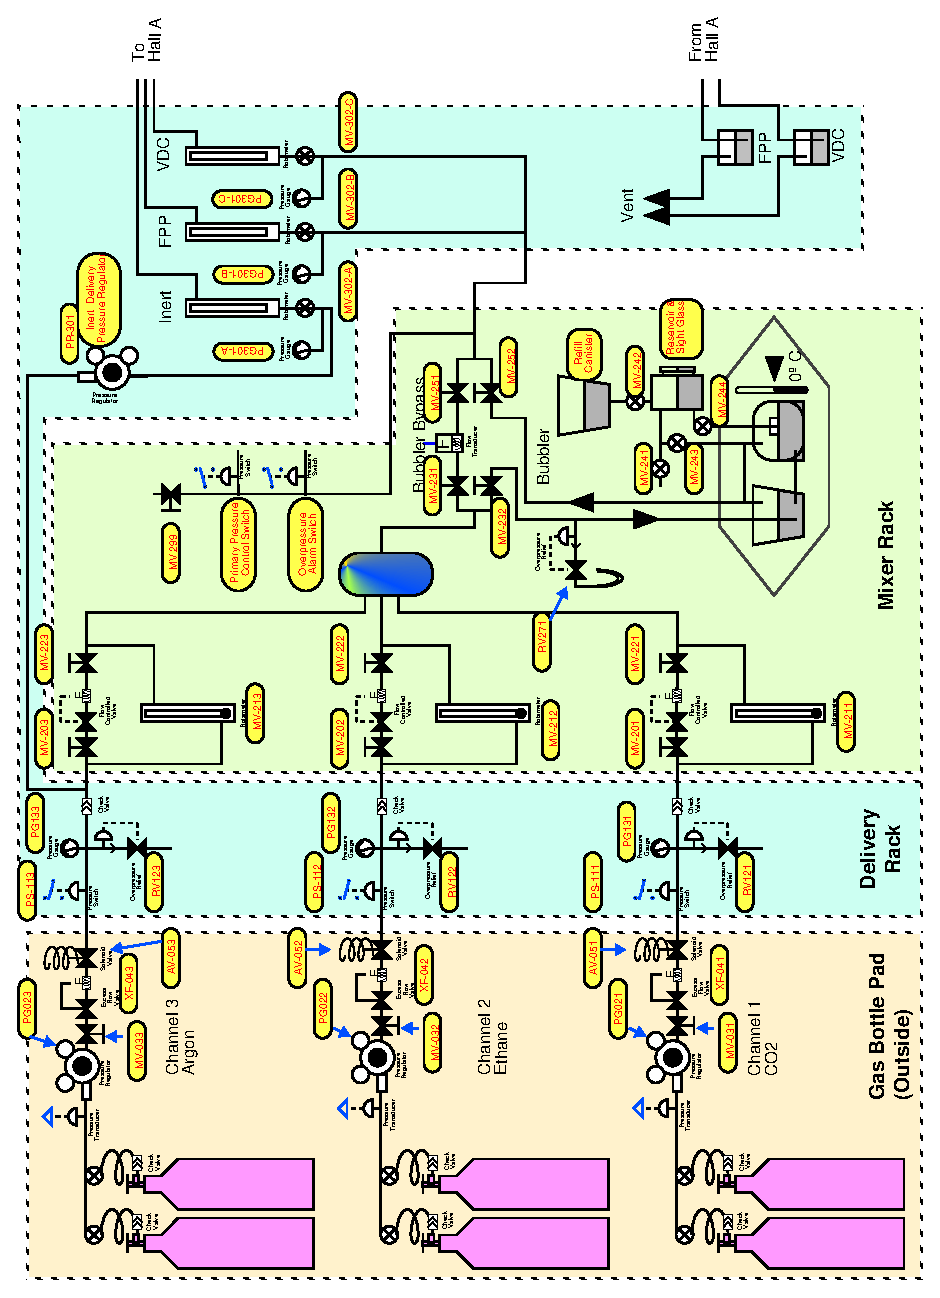
\includegraphics[angle=0,width=15cm]{gas_shed_schematic}
\caption[Gas: shed diagram]{
   Shed Schematic Diagram
}
\label{fig:gas_schem}
\end{center}
\end{figure}

\section{Gas Mixing Station}
The gas mixing system works by metering three gas supplies into a
common mixing tank.  The mixture is then bubbled through alcohol in a
tank within a small refrigerator which has been modified for safe
operation in a flammable gas system. Because the gas {\it flow}, not
the pressure, is regulated by the metering system, pressure switches
have been installed to monitor the mixer outlet pressure and provide
feedback to the flow-control system. The mixing, bubbling, and
pressure control systems are all built into the same relay rack.  They
are collectively referred to as the Gas Mixing Station.  A flow
diagram is shown in Figure\ref{fig:gas_schem}

\subsection{ Mass Flow Control System}
The flow rate of each component gas is controlled by a mass flow
controller which delivers a constant mass of gas per unit time.
(Tylan General model FC-280AV) The mass flow is independent of
pressure, although a minimum differential pressure across the
controller is required for proper operation.  The valves are
factory-calibrated for Nitrogen (N$_2$).  The system controlling them
is field-programmed to compensate for different gasses.  Flow channel
1, currently assigned for CO$_2$, has a mass flow controller
calibrated to deliver a maximum of 100 sccm (standard cubic
centimeters per minute) N$_2$ (74 sccm CO$_2$).  Flow channels 2 and 3
have controllers with a full scale range of 1000 sccm N$_2$.  With the
calibration factors taken into account the maximum flows are 500 sccm
Ethane (channel 2) and 1450 sccm Argon (channel 3). Manual valves
(MV-201 \& 221, etc.) are provided which allow one to bypass the mass
flow controllers and use a needle-valve / rotameter set (MV-211, -212,
-213) if desired.  The needle valve must be closed during normal
operation using the mass flow controllers.

\begin{figure}[htp]
\begin{center}
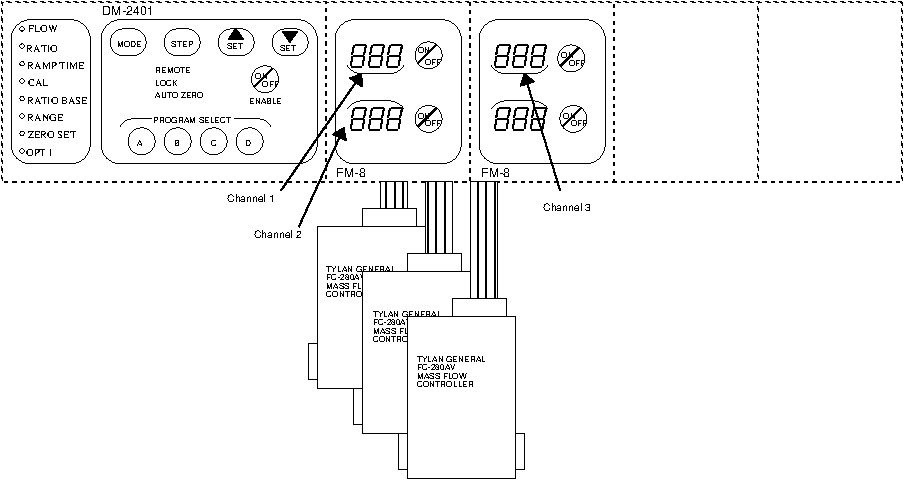
\includegraphics[angle=0,width=15cm]{gas_dynamass}
\caption[Gas: mass flow control]{
   Block Diagram of Mass Flow Control System.
}
\label{fig:gas_massflow}
\end{center}
\end{figure}

The mass flow valves are controlled by a Dynamass Flow Control System
(Vacuum General, Inc. model DM-2401). This unit is outfitted with four
flow-control channels (two model FM-8 two-channel modules) and could
be upgraded to eight flow channels if desired. Refer
Figure\ref{fig:gas_massflow} for a diagram of this system.  Currently
HAWGS has only three of the four channels instrumented.  The FM-8
receives a flow measurement from its associated flow controller,
adjusts it by the calibration factor for the gas being used, and
displays the result on the front panel.  If the measured flow differs
from the desired flow as set in the FM-8 by an operator, a correction
signal is sent to adjust the valve in the flow controller.  The
DM-2401/FM-8 system allows the user to define up to four mixture/flow
settings.  Refer to the Dynamass System manual and to section 3.3.3
{\it Setting a Flow Rate} for more detail on operating the flow
controllers.

The measured flows of the three component gasses are combined in a
small blending tank in the back of the mixing station.  The resulting
mixture is delivered to the alcohol bubbler through a line which is
teed to an overpressure relief valve (RV-271) set for 25 psig.  This
prevents overpressuring of the blending tank, the bubbler, or the
delivery lines.

\subsection{ Alcohol Bubbler}
  
\begin{figure}[htp]
\begin{center}
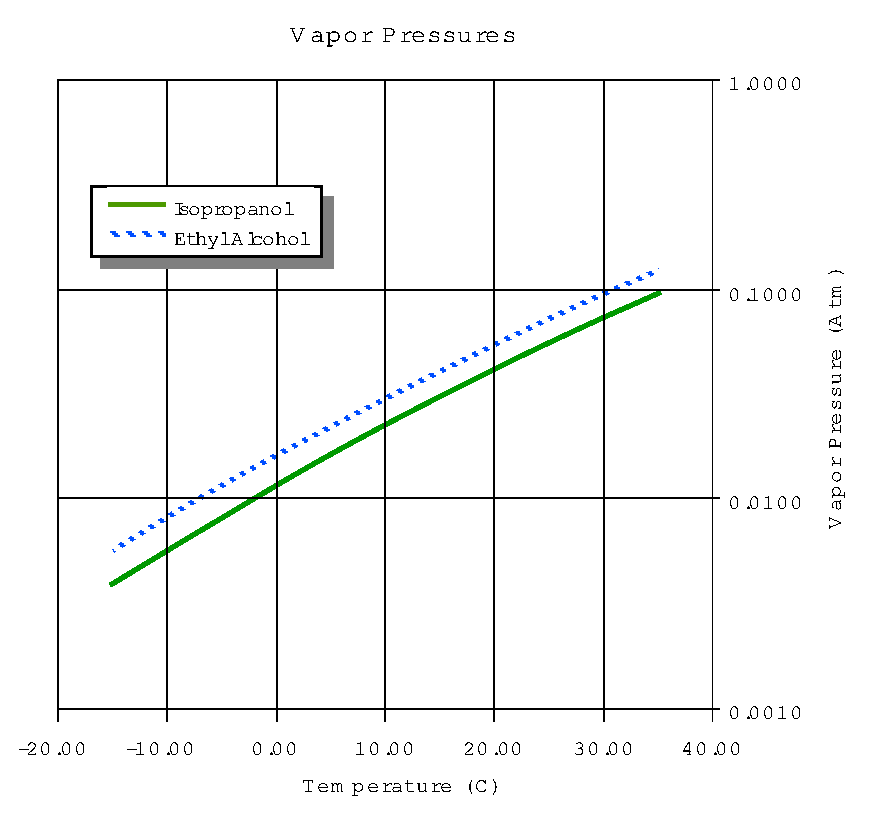
\includegraphics[angle=0,width=15cm]{vap_press}
\caption[Gas: Vapor pressure]{
   Vapor Pressures of Isopropyl and Ethyl Alcohols 
   calculated using the CRC Handbook parameterization.
}
\label{fig:gas_vap}
\end{center}
\end{figure}

Because the interesting alcohols for use in wire chambers have a
feeble vapor pressure at room temperature, it is not convenient to
purchase bottled gas with alcohol already added.  A practical means of
adding alcohol vapor to a gas is to pass the gas through a reservoir
of the liquid alcohol which is maintained at a specified temperature.
At a given temperature, the vapor pressure of the alcohol may be
known, and this vapor pressure represents directly the partial
pressure of the vapor in the gas mixture.  The vapor pressures of
organic compounds may be calculated from information in the CRC
\underline{Handbook of Chemistry and Physics}, where it has been
parameterized as
\begin{equation}
Log10 P = (-0.2185 A/K) + B
\end{equation}

where P is the pressure in Torrs, K is the temperature in Kelvin, and
A and B are parameters provided in the Handbook for a number of
compounds.  For isopropanol within the temperature range -26.1$^o$C to
+232.0$^o$C, the parameters given are A=10063.5 and B=8.996156.  For
Ethyl Alcohol the parameters are A=9673.9, B=8.827392.

At 0$^o$C, for example, this formula gives the vapor pressure of
isopropanol as 0.0115 Atm.  (1 Atm. � 760 Torr).  If the gauge
pressure of the bubbler gas + vapor is 1 atmosphere (2 Atm absolute
pressure), as intended for Hall A, then the fraction of alcohol vapor,
by partial pressure, is about 0.57\%. Figure~\ref{fig:gas_vap} shows the
vapor pressures of these alcohols as a function of temperature.

Note that the bubbler temperature defines the vapor pressure and thus
the �dew point� for the vapor in the gas.  If the gas comes in contact
with any surface which is colder than the dew point (the temperature
of the bubbler) the alcohol vapor will condense on that surface.  This
is why it is important that all components of the gas system be
maintained at a temperature above that of the alcohol bubbler.
Because gas in the Hall A chambers is at about 1 atmosphere absolute
pressure while that in the bubbler is at twice this pressure, the dew
point for the gas in the chambers is lower than the bubbler
temperature.  The bubbler system consists of a refrigerator, a bubbler
tank, a cold reservoir, a warm reservoir, and a fill tank.  A float
valve automatically maintains the liquid levels in the bubbler tank
and the cold reservoir.  Alcohol enters the bubbler tank only from the
cold reservoir so that its temperature has already been established.
The warm reservoir, sitting above the refrigerator, is equipped with a
sight glass and serves as the main on-line alcohol storage vessel.
When the level of liquid in this tank becomes low it must be manually
refilled from commercially supplied bottles using the fill tank.  The
refrigerator used to maintain the alcohol bubbler temperature has been
modified specifically to make it safe for containing flammable gasses
and liquids.

Filling the alcohol reservoir is not trivial.  Please refer to and
carefully follow the procedure detailed in section 3.3.2 {\it Adding
Alcohol}.

\subsection{ Delivery Pressure Control}
Gas will be metered to each detector element through a needle valve.
To achieve a constant flow through a needle valve a constant
differential pressure must be maintained across it, so it is necessary
to provide a fairly constant supply pressure out of the mixing
station.  This comes only at a price, as the mass flow controllers
deliver a fixed {\it flow rate} regardless of pressure (within
practical limits).  If the detectors in Hall-A consume less gas than
the mixer supplies, the pressure in the supply lines will increase.
Similarly, if less gas is mixed than is consumed the pressure will
decrease.  To provide a usefully constant pressure of about 15 psig in
the supply line, a pair of pressure switches has been installed in the
mixing station outlet.  The first of these, the {\bf Primary Pressure
Control Switch}, is set to open at 16 psig and close again at 14 psig
or below.  When the pressure is low this switch is closed and the Flow
Control System is commanded to use the flow rates set into its PROGRAM
C ("high flow").  When the {\bf Primary Pressure Control Switch}
opens, PROGRAM-D ("zero flow") is selected.  By setting PROGRAM-C to
provide just a little more gas than required by the detectors, the
supply pressure can be maintained at between 14 and 16 psig. with a
cycle time of several minutes.  This pressure variation will result in
a flow rate variation of no more than about 15\%, which should be of
no consequence for the detectors.

A second pressure switch, the {\bf Overpressure Alarm Switch}, is
calibrated to open at 18 psig and re-close at 14 psig or below.  If
the delivery line pressure manages to exceed the 18 psig threshold it
indicates a system failure of some sort and the gas interlock system
is tripped by this switch.  Manual operator intervention is then
required to re-establish gas flow.

Pressure control of the inert gas supply, used to purge the detectors,
is provided by a conventional single-stage regulator (PR-301) mounted
inside the delivery rack.  This regulator receives 45 psig inert gas
(the same gas delivered to mixer flow channel 3) and provides 15 psig
gas to the INERT supply line to Hall-A.

\section{Gas Delivery into Hall A}

Between the gas shed and the two Hall-A shield houses are several gas
line runs of about 700 feet in length.  These are shown schematically
in Figure~\ref{fig:gas_dist}. Three gasses (inert, VDC, and FPP) are
supplied to the Hadron Arm through 1/2-inch OD polyethylene tubing.
Two similar tubes are teed into these near the beamline entrance to
Hall-A and they supply VDC and inert gas to the Electron Arm shield
house.  The pressures in all of these lines is nominally 15 psig.

\subsection{ Distribution in the Shield Houses}

Inside each shield house there is a gas distribution panel which
controls the gas flows to the individual wire chambers in that
detector stack.  Figure~\ref{fig:gas_dist} shows a diagram of the shield
house gas systems.

Each gas supply is first filtered and fed to a visual pressure gauge
(PG-401-A/B and PG- 501-A/B/C) so that the supply pressure can be
locally verified.  Inert gas (for purging detectors) and operating gas
(either VDC or FPP gas) is manifolded to a series of three-way valves
� one for each detector flow circuit.  These valves are labeled
MV-411, -412 in the Electron Arm, and MV-511 � MV-516 in the Hadron
Arm.

The three-way valve associated with each detector may be used to
select either operating or purge gas independently of the other
detectors.  The selected gas is supplied to the inlet of a
needle-valve / rotameter combination (labels MV-42x and MV-52x) which
is to be used to set and observe the gas flow to each detector.  The
rotameters are sized for reasonably accurate metering of 5 slph
Argon-Ethane and purging at about ten times this rate.  (Note that the
gas mixer will supply a total of only 60 slph Argon-Ethane, limited by
the capacity of the Ethane mass flow controller).

On its way from the rotameter to the detector the gas passes by an
overpressure relief bubbler which is basically a manometer filled with
mineral oil.  The overpressure bubblers are set to release at a
pressure greater than about 30 mm of water ($\sim$33 mm mineral oil).
This pressure is sufficient to allow purging at the desired rate.  Gas
returning from the detector passes through an electronic mass flow
meter and through a low pressure oil bubbler.  This bubbler prevents
backstreaming of waste gas into the detectors.  The flow meter reading
is indicated locally on a LCD display and is available as an analog
signal for connection to the slow controls computer.  Note that these
digital flowmeters are factory- calibrated for Nitrogen.  To correct
the readings for Argon multiply by 1.45; for Ethane multiply by 0.5;
for CO$_2$ multiply by 0.74.

\subsection{ Waste Gas Collection and Venting}
Gas coming from the chamber exhaust bubblers is collected in a
manifold and routed back to the gas shed through a large (1-inch OD)
polyethylene tube.  There are separate manifolds and exhaust lines for
the VDC and FPP systems.  Back-pressure in the exhaust manifolds is
monitored by PHOTOHELIC${(R)}$ pressure switches.  If more than about
1-inch H$_2$O backpressure develops in an exhaust manifold the gas
supply interlock system is tripped, turning off the gas supply at the
solenoid valves outside the gas shed.  The purpose of this particular
interlock is to protect the detector windows from overpressure.

\begin{figure}[htp]
\begin{center}

\includegraphics[angle=0,width=15cm]{blank}
\caption[Gas: Hall A]{
   Gas Distribution inside Hall-A.
}
\label{fig:gas_dist}
\end{center}
\end{figure}


\section{Autherized Personnel}
The following personnel are responsible for problems concerning the
gas system:

\begin{itemize} 
\item[~]Howard Fenker -x7431
\item[~]Jack Segal -x7242
\end{itemize} 


\section{Safety and Device Protection}

There are a number of monitor points which provide signals to the gas
interlock panel and which can cause the supply of gas to be
interrupted.  The primary purpose of this system is to facilitate the
safe handling of a flammable gas.  A secondary but equally important
function is protection of the detector hardware.  Finally, this system
serves to help insure the integrity of the data collected by Hall A
experiments by alerting the experimenters on shift if a condition
arises which might affect the detector gas quality.  The conditions
monitored are 1) flammable gas leak detection, 2) low main supply
pressure, 3) high delivery pressure, 4) high exhaust line pressure, 5)
forced airflow in gas shed, 6) over-temperature in gas shed or a
shield house, and 7) house fire alarm.  The "Kill Gas" buttons in the
counting room and in the gas shed also feed into this interlock
system.


When a fault condition occurs, power to the solenoid valves
controlling gas flow into the gas shed is turned off, closing the
valves.  An audible alarm sounds in both the gas shed and the counting
room, and one or more red lights on the interlock panels in both
locations indicate the specific fault detected.  The audible alarm may
be silenced by pressing the "Alarm Override" button.  Note that this
does not restore gas flow or clear a fault.

After the fault is cleared it is necessary to activate the "Low
Pressure Override" circuit by pressing the corresponding button on the
interlock panel in the gas shed.  This circuit temporarily disables
the "Low Pressure" fault circuit, allowing the solenoid valves to open
up and restore gas pressure to the inlet pressure switches.  When
pressure is restored this circuit automatically resets itself.

Note that the {\bf Excess Flow Valves} will almost always trip
immediately after the solenoid valves are re-opened.  This is because
of the sudden high flow rate which occurs when the pressure in the gas
line downstream of a solenoid valve is low and the solenoid valve is
opened with full inlet pressure. To reset the {\bf Excess Flow Valves}
refer to the section {\it Resetting a closed Excess Flow Valve}.

\section{System Operation}

\subsection{ Pre-Startup Checklist}

Before initial use with a flammable gas or after a significant
down-time the following checks should be made to insure the safety and
integrity of the HAWGS:

\begin{enumerate}
\item Leak-Check the entire gas system using a �safe� gas such as Argon or Nitrogen.
\item Calibrate over-pressure relief valves: RV121, 122, 123 should release at 55-65 psig, 
RV271 must release at 20-25 psig).
\item Check calibration of Excess-Flow valves (should close at 4-5 slpm).
\item Check proper operation of each interlock circuit and that interlock system shuts off gas 
supply.
\item Measure the detectors leak rates and verify that each is below 7 slph (or current 
administrative limit - note that current physical limit is 500 sccm
Ethane and 1450 sccm Argon based on flow controller full scales for
N$_2$ and correction factors for Ethane and Argon).
\item Verify that flammable gas leak sensors are appropriately calibrated.
\end{enumerate}

\subsection{ Startup Procedure}

\begin{enumerate}
\item Close gas shed outlet valves MV-302-A, -B, -C to isolate the mixing/delivery system 
from the spectrometer detectors.
\item Activate the "Kill Gas" crash button.  Interlock panel should alarm.  Silence the alarm 
by pressing "Alarm Silence". Reset the Crash Button by pulling outward. If any fault 
conditions (red LED) other than "Low Pressure" and "Main Relay" are indicated, clear 
them by correcting the indicated fault.
\item Check alcohol supply and Bubbler temperature.  Fill and/or adjust as 
necessary (see  {\it Adding Alcohol}) .
\item Check that adequate supply bottles of appropriate gasses are attached to the high 
pressure supply manifolds and valve {\bf one} bottle ON for each manifold.
\item Verify that all used main pressure regulators (outside) are set for 45-50 psig.
\item Select "Manual / Expert" pressure control using toggle switch on panel in rear of 
mixing station, behind flow controller.  {\bf Note that while in 
"Expert" mode there 
is no automatic delivery pressure control!}  Overpressure is prevented only by 
the overpressure shutoff switch and the alcohol reservoir relief valve.
\item Verify that the Dynamass Flow Control System DM-2401 is in 
"Non-VG" mode by 
\begin{itemize}
\item Press PROGRAM SELECT pushbutton �A�.
\item Put the DM-2401 in �NO-MODE� mode (if it is not already) by pressing the 
MODE pushbutton until all LED�s in the column of LED�s on the left of the unit 
are off.
\item Simultaneously press and release PROGRAM SELECT buttons �A� and �C�.
\item Press the MODE pushbutton until the �OPT 1� LED is lighted.  Verify that the 
display for channel 4 reads all zeros.
\item Return the DM-2401 to �NO-MODE�.
\end{itemize}
\item Set Dynamass Flow-Control System to Program "D: Zero Flow".  Put the DM-2401 in 
"FLOW-MODE" and verify that all flow settings are at zero. 
\item With the DM-2401 in "FLOW-MODE", set up flow program "C" to provide the desired 
mixture at about 10\% higher total flow than the detectors are expected to consume.
\item Return the DM-2401 to "NO-MODE".
\item Select "Auto" pressure control using toggle switch on panel in rear of mixing station, 
behind flow controller.
\item Actuate the Low Pressure Override on interlock panel.  "Main 
Relay" light should 
become green.
\item Set Excess-Flow Valves and Manual valves at regulators to full OPEN, wait about ten 
(10) seconds for supply lines to come up to pressure, then set all three Excess Flow 
Valves to AUTO SHUTOFF. - "Low-Pressure" interlock circuit should go to green 
during this step$^3$.
\item Verify proper operation of flow/mix control system and outlet pressure regulation by 
observing flow rates on the mixer control and outlet pressure at the supply rack 
(pressure gauges 301B, -301C). If the alcohol bubbler loop is valved on it may take 
several minutes for its volume to fill with gas and come up to pressure. Be patient. 
When the pressure indicated on gauges PG301-B/C reaches about 15 psig the DM2401 
system should cycle to flow program D. To bleed down the outlet pressure in order to 
cause the pressure loop to cycle, you may crack valve MV-299 (located in the rear of 
the mixer rack). When the pressure drops back to about 13 psig the control system 
should switch back to program C. Re-close valve MV-299 when tests are complete.
\item Check/Adjust the Purge gas pressure regulator (PR 301) to insure that the delivery 
pressure of the inert gas (taken from gas supply 3 - nominally Argon) is about 15 psig 
as registered on pressure gauge PG-301A.
\item Slowly open gas shed outlet valves MV-302-A, -B, -C to bring up the pressure in the 
supply lines to the spectrometers.  After pressure has equalized open these three valves 
fully.  Note that one or more {\bf Excess Flow Valves} will trip (close) if the 
{\bf total} gas flow 
through the three rotameters associated with these valves exceeds (roughly) 150 units 
(full scale on {\bf one} rotameter).

\item At each of the Hadron and Electron shield house gas distribution racks, verify the 
presence of supply pressures (gauges PG401A,B and PG501A,B,C) and set gas 
selection valves and needle valves to desired gasses and flow rates for each chamber.
\end{enumerate}
\subsection{  Normal Operation}
\subsection{ Changing gas bottles}

{\bf Warning: High pressure gas bottles contain significant stored energy and 
are potentially hazardous.  Handling of gas bottles should be done only by 
qualified, trained personnel.}

For smoothest operation, used gas bottles should be replaced before their internal pressure 
drops below the desired regulator output pressure.  

The sequence of steps for replacing an empty gas bottle is as follows:
\begin{enumerate}
\item Make sure that the backup bottle is full, then open its bottle valve and its manifold 
valve.  The in-line check-valves will prevent back-filling of the empty bottle.  As a 
precaution, set the corresponding {\bf Excess Flow Valve} to {\bf 
OPEN/RESET}, wait ten seconds, 
then set the {\bf Excess Flow Valve} back to {\bf AUTO}.
\item Close both the bottle and manifold valves for the empty bottle.
\item Disconnect the empty bottle from the high-pressure flex-line, replace the bottle�s cap, 
and move the empty bottle to the EMPTIES storage rack.  Note that ethane bottle 
fittings, type CGA-350, have left-handed threads.
\item Place a full bottle of gas in the on-line rack, remove the bottle cap,  and connect the 
bottle to the flex-line.
\item Open the new bottle�s valve, check for leaks at the bottle fitting, then re-close the bottle 
valve.
\end{enumerate}

\subsection{ Adding Alcohol}

{\bf Warning: Never open gas flow into the alcohol bubbler without an outlet 
valve being open.}

As long as the level in the {\bf RESERVOIR} is such that some alcohol is visible in the sight glass 
the bubbler will be maintained at its normal fill.  An effort should be made to prevent the 
{\bf RESERVOIR} level from getting too low.

\begin{enumerate}
\item To fill the {\bf RESERVOIR} close valves MV-243 and MV-244 to isolate the RESERVOIR from 
the pressure equalization line.  
\item Open valve MV-241 to vent the {\bf RESERVOIR. } 
\item Remove the cover of the {\bf REFILL CANISTER} and fill the canister with alcohol. Put the 
cover back on but do not seal it (if you seal the cover at this point the flow of alcohol 
out of the {\bf REFILL CANISTER} will be impeded).  
\item Open valve MV-242 to let the alcohol into the {\bf RESERVOIR}.  The liquid level can be 
monitored in the sight glass on the side of the {\bf RESERVOIR}.  Fill until the liquid level is 
near the top of the sight glass then close MV-242.  {\bf Do not 
overfill} (to or above the top of the sight glass).  
\item Close valve MV-241, then open valves MV-243 and MV-244.
\item Seal the cover on the {\bf REFILL CANISTER} to prevent contamination.
\end{enumerate}

\subsection{ Setting a Flow Rate}

The flow of each individual gas component, and therefore the final gas mixture, is 
controlled by the {\bf Dynamass DM-2401 System}, the {\bf FM-8 Flow/Ratio 
Modules}, and the {\bf Tylan General 
FC-280 Mass Flow Controllers}.  The {\bf DM-2401} accepts and stores programs 
for the set of {\bf FM-8's}.  
Each {\bf FM-8} controls one or two {\bf Mass Flow Controllers}.
 
To set or alter a flow rate:
\begin{enumerate}
\item Prevent the mixed-gas outlet pressure from exceeding its 18 psig interlock trip level by 
either a) closing valves MV-201,2,3, or b) insuring that the detectors are consuming a 
sufficient quantity of gas to prevent this overpressure from occurring during the time it 
takes you to perform steps 3-11, below.
\item Set the Auto/Expert pressure control switch (rear of mixer rack) to EXPERT.
\item Verify that the DM-2401 is in the NO-MODE mode, indicated by none of the LED�s in 
the column on the extreme left of the unit being illuminated.  If necessary, press the 
MODE pushbutton until this condition is achieved.
\item Press program select button �C� and verify that the corresponding LED illuminates. 
\item At the DM-2401 Keyboard module, press the MODE switch until the FLOW LED 
illuminates.  The window value for channel 1 will begin to flash.
\item Select the channel you wish to alter by pressing the STEP button until the window 
value of the desired channel is flashing.
\item Press the UP or DOWN SET buttons to alter the value as desired.  Legal flow values 
are 0.0-100.0 sccm for channel 1, 0-1000 sccm for channels 2 and 3.
\item If the Red �ON� LED for the desired channel (immediately to the right of the value 
window) is not lit, press the ON/OFF button for that channel to illuminate this LED.
\item Repeat steps 6-8 as necessary to program all desired gas flows.
\item Return the DM-2401 to NO-MODE as in step 3.
\item Return the Auto/Expert pressure control switch (rear of mixer rack) to AUTO.
\item Re-Open valves MV201, 202, 203, if closed in step 1.
\item Observe system flow and pressure control and verify that it is correct.
\end{enumerate}

\section{Troubleshooting :  Things to Check}

Each of the following monitor points must report a nominal condition to the gas interlock 
panel in order for the logic to be "made up" and for gas flow to be enabled:

\begin{tabular}{|l|l|l|l|}
\hline
{\bf Label} & {\bf Meaning} & {\bf Likely Remedy} & {\bf Sensor} \\
\hline
Low Pressure & The seconeary & $\bullet$ Check for a closed & 3 pressure \\
Note: {\it This channel} & pressure of one or & "Excess Flow" Valve, & 
switches located \\
{\it will always indicate} & more of the mixer & Remedy the cause, and & 
on the "Delivery \\
{\it a fault after some} & inlet gas supplies & reset the valve & Rack" 
\\
{\it other problem has} & has dropped below & $\bullet$Replace empty 
supply & {} \\
{\it caused the solenoid} & the 45 psi & bottle. & {} \\
{\it valves to close.} & threshold. & {} & \\
\hline
Gas Shed Airflow & Gas Shed Exhaust & Restore forced & Vane Switch \\
{} & Fan ( ceiling of & ventilation. & mounted just \\
{} & "Isobutane Room') & {} & inside exhaust \\
{} & has failed. & {} & fan \\
\hline
Overtemp Gas Shed & Temperature in Gas & $\bullet$Take action to protect 
& Klixon mounted \\
{} & Shed Too High & equipment. & in rack \\
{} & ($\sim$110$^o$F). & $\bullet$Reduce temperature. & \\
\hline
Over-Pressure FPP & VDC/FPP Exhaust & $\bullet$Eliminate exhuast line & 
PHOTOHELIC$^{(R)}$ \\
Over-Pressure VDC & manifold pressure & blockage & gauges on gas \\
Electron & at Hadron Or & $\bullet$Allow Hall-A & panels in shld \\
Over-Pressure VDC & Electron Shield & atmospheric pressure to & houses \\
Hadron & House Gas Rack & stabilize & {} \\
\hline
Gas Leak & Flammable gas & $\bullet$Localize leak by & GASMASTER \\
{} & detection system & referring to readings on & HydroCarbon \\
{} & has sensed a leak & GasMaster-4 system in & Detector heads in \\
{} & {} & Counting House & Gas Shed and \\
{} & {} & $\bullet$Fix Leak & each Shield \\
{} & {} & {} & House. \\
\hline
Overtemp Electron & Temperature in & $\bullet$Take action to protect & 
Klixon mounted \\
{} & Electron Shield & equipment. & in gas rack in \\
{} & House Too High & $\bullet$Reduce temperature & Electron Shield \\
{} & ($\sim$110$^o$F). & {} & House \\
\hline
Overtemp Hadron & Temperature in & $\bullet$Take action to protect & 
Klixon mounted \\
{} & Hadron Shield & equipment. & in gas rack in \\
{} & House Too High & $\bullet$Reduce temperature. & Hadron Shield \\
{} & ($\sim$110$^o$F). & {} & House \\
\hline
Post-Bubbler & Gas pressure out of & $\bullet$Reset Dynamass & Pressure 
switch \\
Supply & mixer/bubbler rack & Controller & in rear of Mixing \\
Overpressure & is $>$18 psi. & $\bullet$If needed, vent excess & Station 
\\
{} & {} & pressure using MV-299 & (mixer/bubbler \\
{} & {} & {} & rack) \\
\hline
\end{tabular}

\subsection{ Resetting a closed Excess Flow Valve}

Each Excess Flow Valve automatically closes if the flow rate through it 
exceeds about 4 slpm at 45 psig.  The exact flow threshold varies somewhat 
depending upon the delivery 
pressure.  

\vspace{0.25in}                        

These valves must be manually reset after they trip.  This is done by
rotating the red handle 90$^o$ CW (to OPEN/RESET ) and then 90$^o$ CCW
(back to AUTO SHUTOFF. ).  It will be necessary to keep the valve in
the OPEN/RESET position for about 10 seconds until nominal pressure
builds up downstream.  The excess flow valves must be returned to the
AUTO SHUTOFF setting to insure system safety.

\leftline{ \bf Restoring flow after a "Low Supply Pressure" shutdown}

If the gas pressure in any enabled supply line to the mixer rack drops
below about 40-45 psig, the interlock will sound an alarm and close
all of the solenoid valves.  This prevents the system from delivering
a bad mixture to the detectors. After restoring the gas supply, for
example, after replacing an empty gas cylinder, perform the following
steps to restart the flow of gas.
\begin{enumerate}
\item Verify that no faults other than "Low Pressure" and "Main Relay" are 
indicated on the gas interlock panel.
\item Insure that all high-pressure manifolds are pressurized and that the 
secondary pressures indicated by the gauges above the bottles are at
about 40-45 psig (normally these should not need adjustment).
\item Press the Low Pressure Override button on the interlock panel in the gas 
shed.
\item Reset all Excess Flow Valves by turning their handles to OPEN/RESET, 
waiting for about ten seconds, then returning their handles to AUTO
SHUTOFF.
\item Verify that all faults are now cleared on the gas interlock panel.
\end{enumerate}

\subsection{ Restarting flow after a power failure.}

Normally the gas control system is protected from power outages by an
uninterruptable power supply (UPS).  If the system is nevertheless
disturbed by a loss of power then perform the steps outlined in
section 3.2, Startup Procedure.

\section{Maintenance}
\subsection{ Periodic Inspections}

Anytime work is done on any part of the gas system, or there is an
occurrence that could possibly have damaged the gas system, the system
should be carefully inspected and checked for leaks.

The flammable gas detector heads and control system should be tested
periodically for proper operation, in accordance with the
manufacturer's recommendations and the TJNAF fire safety program.

Each sensor feeding the Gas Interlock Panel should be exercised at
least annually for proper operation.  The interlock system itself
should be tested at the same time to insure that it interrupts the
supply of gas when it is tripped.

The high-pressure manifold and bottle connections should be regularly
checked for leaks and damage.  In particular, the CO$_2$ system
(CGA-320) uses plastic seals at the bottle connection which must be
replaced periodically.

\paragraph{\bf Flowmeter Calibration}

The Tylan General mass flow controllers (mass flow valves) require
periodic cleaning and calibration (section 5.7, Tylan General Mass
Flow Controller Instruction Manual ).  The first step in this process
is to check the operation of the instruments and perform further work
as necessary.  This procedure should be planned and carried out
whenever 1) there appears to be a problem with the operation of a flow
controller, or 2) there is a lengthy break in the Hall-A program that
would allow the gas system to be taken off-line for several weeks.  If
absolutely necessary the needle-valve/rotameter combinations plumbed
in parallel with the mass flow controllers could be used to allow
interim operation of the gas system while one or more flow controllers
is removed for maintenance.

